\documentclass{article}
\usepackage[utf8]{inputenc}
\usepackage{amsthm,amsmath,bm,bbm}
\usepackage{amssymb,mathtools}
\usepackage[dvipsnames]{xcolor}
\usepackage[colorlinks=true, allcolors=violet]{hyperref}
\usepackage{tikz}
\usetikzlibrary{shapes,shadows,arrows,positioning,arrows.meta,decorations.pathreplacing,decorations.pathmorphing,decorations.shapes}
\usepackage[colorinlistoftodos,textsize=scriptsize,textwidth=.8in,color=blue!20]{todonotes}

\begin{document}

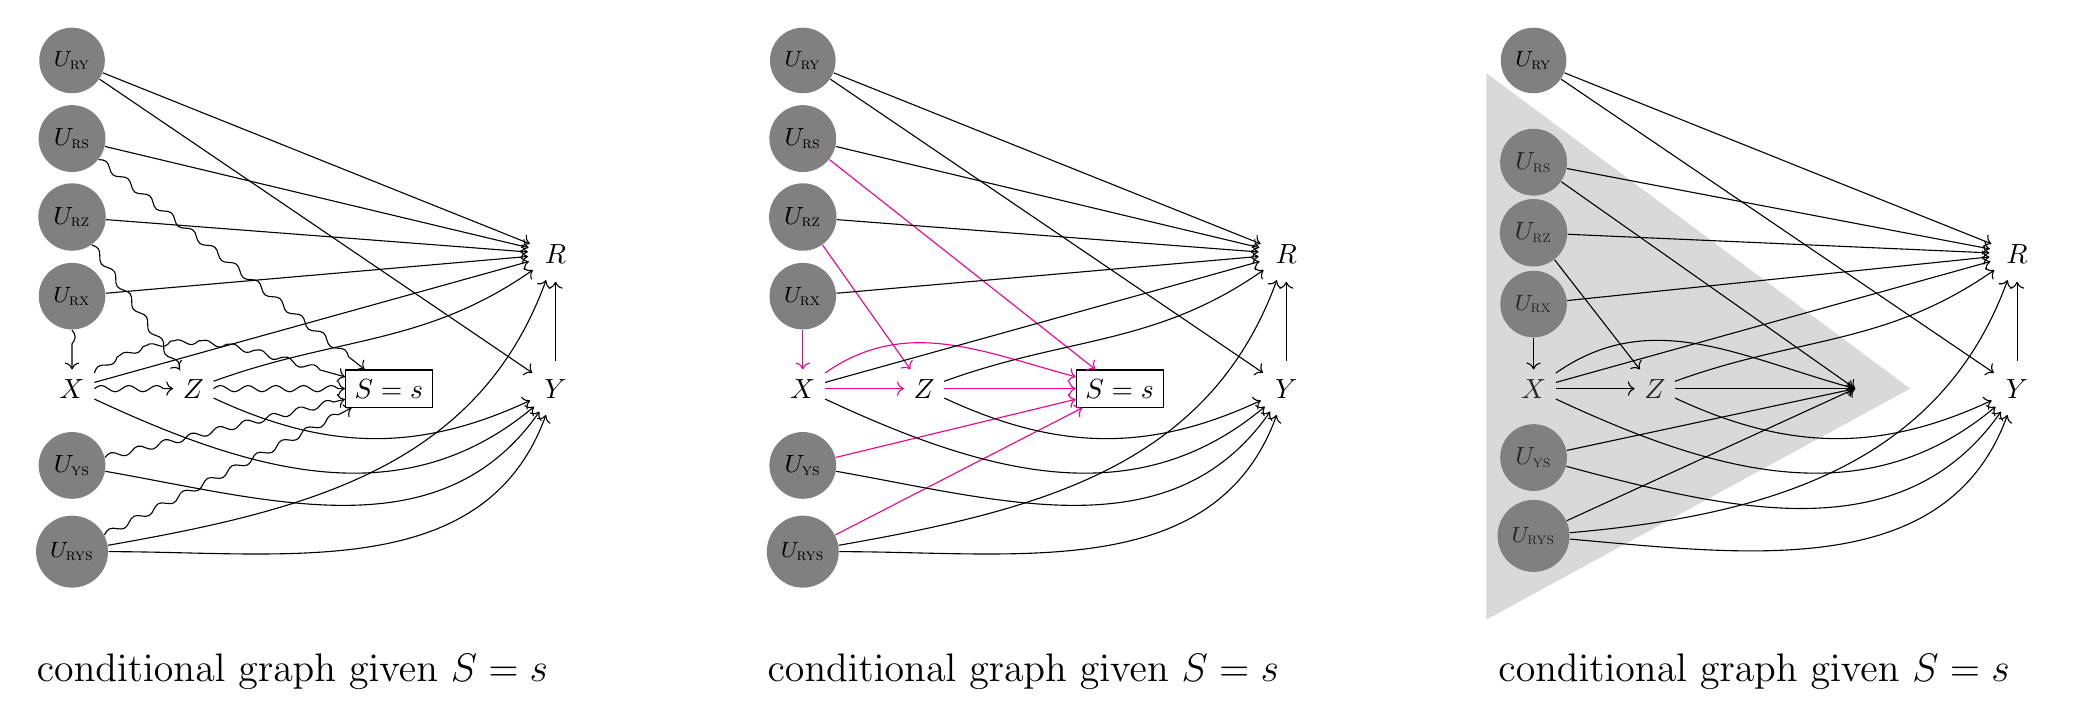
\begin{tikzpicture}[
    v/.style={rectangle, minimum width=1mm, minimum size=1mm, text centered},
    c/.style={circle, fill = gray!20},
    u/.style={circle, fill = gray},
    o/.style={circle}]
        
        % DM %%%%%%%%%%%%%%%%%%%%%%%%%%%%%%%%%
        \node[v] (X)                                 {$X$};
        \node[v] (Z)    [right=of X]                {$Z$};
        \node[o] (Y)    [right=of X,   xshift=45mm] {$Y$};
        \node[v,draw] (S)    [left=of Y, xshift=-2mm]                 {$S=s$};
        \node[u] (Uys)  [below=of X,   yshift=7mm]  {\small $U_\textsc{ys}$};
        \node[u] (Urys) [below=of Uys, yshift=8mm]  {\footnotesize $U_\textsc{rys}$};
        
        \node[o] (R)   [above=of Y]                 {$R$};
        \node[u] (Urx) [above=of X, yshift=-5mm]    {\footnotesize $U_\textsc{rx}$};
        \node[u] (Urz) [above=of X, yshift=5mm]     {\small $U_\textsc{rz}$};
        \node[u] (Urs) [above=of X, yshift=15mm]    {\small $U_\textsc{rs}$};
        \node[u] (Ury) [above=of X, yshift=25mm]    {\footnotesize $U_\textsc{ry}$};
        
        \draw[->, decorate, decoration={coil,aspect=0,amplitude=.4mm}] (Urx) -- (X);
        
        \draw[->, decorate, decoration={coil,aspect=0,amplitude=.4mm}] (X)   -- (Z);
        \draw[->, decorate, decoration={coil,aspect=0,amplitude=.4mm}] (Urz) -- (Z);
        
        \draw[->, decorate, decoration={coil,aspect=0,amplitude=.4mm}] (X)    to[out=35,in=165] (S);
        \draw[->, decorate, decoration={coil,aspect=0,amplitude=.4mm}] (Z)    --                (S);
        \draw[->, decorate, decoration={coil,aspect=0,amplitude=.4mm}] (Uys)  --                (S);
        \draw[->, decorate, decoration={coil,aspect=0,amplitude=.4mm}] (Urys) --                (S);
        \draw[->, decorate, decoration={coil,aspect=0,amplitude=.4mm}] (Urs) -- (S);
        
        
        \draw[->] (X)    to[out=-25,in=220]  (Y);
        \draw[->] (Z)    to[out=-25,in=-155] (Y);
        \draw[->] (Uys)  to[out=-10, in=235] (Y);
        \draw[->] (Urys) to[out=0, in=250]   (Y);
        \draw[->] (Ury)  --                  (Y);
        
        \draw[->] (X)    --                 (R);
        \draw[->] (Z)    to[out=20, in=215] (R);
        \draw[->] (Y)    --                 (R);
        \draw[->] (Urys) to[out=10, in=250] (R);
        \draw[->] (Urx)  --                 (R);
        \draw[->] (Urz)  --                 (R);
        \draw[->] (Urs)  --                 (R);
        \draw[->] (Ury)  --                 (R);
        
        \node[v] [below=of X, xshift=28mm, yshift=-20mm] {\Large conditional graph given $S=s$};


        % DM %%%%%%%%%%%%%%%%%%%%%%%%%%%%%%%%%
        \node[v] (X)    [right=of Y, xshift=15mm]   {$X$};
        \node[v] (Z)    [right=of X]                {$Z$};
        \node[o] (Y)    [right=of X,   xshift=45mm] {$Y$};
        \node[v,draw] (S)    [left=of Y, xshift=-2mm]                 {$S=s$};
        \node[u] (Uys)  [below=of X,   yshift=7mm]  {\small $U_\textsc{ys}$};
        \node[u] (Urys) [below=of Uys, yshift=8mm]  {\footnotesize $U_\textsc{rys}$};
        
        \node[o] (R)   [above=of Y]                 {$R$};
        \node[u] (Urx) [above=of X, yshift=-5mm]    {\footnotesize $U_\textsc{rx}$};
        \node[u] (Urz) [above=of X, yshift=5mm]     {\small $U_\textsc{rz}$};
        \node[u] (Urs) [above=of X, yshift=15mm]    {\small $U_\textsc{rs}$};
        \node[u] (Ury) [above=of X, yshift=25mm]    {\footnotesize $U_\textsc{ry}$};
        
        \draw[->, magenta] (Urx) -- (X);
        
        \draw[->, magenta] (X)   -- (Z);
        \draw[->, magenta] (Urz) -- (Z);
        
        \draw[->, magenta] (X)    to[out=35,in=165] (S);
        \draw[->, magenta] (Z)    --                (S);
        \draw[->, magenta] (Uys)  --                (S);
        \draw[->, magenta] (Urys) --                (S);
        \draw[->, magenta] (Urs) -- (S);
        
        
        \draw[->] (X)    to[out=-25,in=220]  (Y);
        \draw[->] (Z)    to[out=-25,in=-155] (Y);
        \draw[->] (Uys)  to[out=-10, in=235] (Y);
        \draw[->] (Urys) to[out=0, in=250]   (Y);
        \draw[->] (Ury)  --                  (Y);
        
        \draw[->] (X)    --                 (R);
        \draw[->] (Z)    to[out=20, in=215] (R);
        \draw[->] (Y)    --                 (R);
        \draw[->] (Urys) to[out=10, in=250] (R);
        \draw[->] (Urx)  --                 (R);
        \draw[->] (Urz)  --                 (R);
        \draw[->] (Urs)  --                 (R);
        \draw[->] (Ury)  --                 (R);
        
        \node[v] [below=of X, xshift=28mm, yshift=-20mm] {\Large conditional graph given $S=s$};


        % DM %%%%%%%%%%%%%%%%%%%%%%%%%%%%%%%%%
        \node[v] (X)    [right=of Y, xshift=15mm]   {$X$};
        \node[v] (Z)    [right=of X]                {$Z$};
        \node[o] (Y)    [right=of X,   xshift=45mm] {$Y$};
        \node[coordinate, minimum size=0pt] (S)    [left=of Y, xshift=-7mm]   {};
        \node[u] (Uys)  [below=of X,   yshift=8mm]  {\small $U_\textsc{ys}$};
        \node[u] (Urys) [below=of Uys, yshift=9mm]  {\footnotesize $U_\textsc{rys}$};
        
        \node[o] (R)   [above=of Y]                 {$R$};
        \node[u] (Urx) [above=of X, yshift=-6mm]    {\footnotesize $U_\textsc{rx}$};
        \node[u] (Urz) [above=of X, yshift=3mm]     {\small $U_\textsc{rz}$};
        \node[u] (Urs) [above=of X, yshift=12mm]    {\small $U_\textsc{rs}$};
        \node[u] (Ury) [above=of X, yshift=25mm]    {\footnotesize $U_\textsc{ry}$};

        \node[coordinate] (coord1) [right=of S, xshift=-3mm] {};
        \node[coordinate] (coord2) [above=of Urs, yshift=-3mm, xshift=-6mm] {};
        \node[coordinate] (coord3) [below=of Urys, yshift=4mm, xshift=-6mm] {};



        \fill[opacity=0.3, gray] (coord1) -- (coord2) -- (coord3) -- (coord1) -- cycle;

        
        \draw[->] (Urx) -- (X);
        
        \draw[->] (X)   -- (Z);
        \draw[->] (Urz) -- (Z);
        
        \draw[->] (X)    to[out=35,in=165] (S);
        \draw[->] (Z)    --                (S);
        \draw[->] (Uys)  --                (S);
        \draw[->] (Urys) --                (S);
        \draw[->] (Urs) -- (S);
        
        
        \draw[->] (X)    to[out=-25,in=220]  (Y);
        \draw[->] (Z)    to[out=-25,in=-155] (Y);
        \draw[->] (Uys)  to[out=-15, in=235] (Y);
        \draw[->] (Urys) to[out=-5, in=250]   (Y);
        \draw[->] (Ury)  --                  (Y);
        
        \draw[->] (X)    --                 (R);
        \draw[->] (Z)    to[out=20, in=215] (R);
        \draw[->] (Y)    --                 (R);
        \draw[->] (Urys) to[out=5, in=250] (R);
        \draw[->] (Urx)  --                 (R);
        \draw[->] (Urz)  --                 (R);
        \draw[->] (Urs)  --                 (R);
        \draw[->] (Ury)  --                 (R);
        
        \node[v] [below=of X, xshift=28mm, yshift=-20mm] {\Large conditional graph given $S=s$};
    \end{tikzpicture}

\end{document}